\chapter{Introdução a Física de Neutrinos.}
A partir do final do século XIX a radioatividade começou a ser estudada por grandes cientistas da época como W.C.Roentgen, A.H.Bequerel, Pierre e Marie Curie e E.Rutherford entre outros.
A lei exponencial do decaimento radioativo foi descoberta naquela época.
Em particular três tipos de processo foram identificados: os decaimentos tipo Alfa ($\alpha$), Beta ($\beta$) e Gama ($\gamma$), cada um com sua partícula característica. 
As partículas α são constituídas de dois prótons e dois nêutrons, ou seja, são núcleos de Hélio. 
A radiação $\alpha$ possui um alcance muito curto, logo sua radiação é pouco penetrante, sendo assim elas têm uma maior facilidade em ser blindadas.
A radiação $\gamma$ corresponde a emissão de um fóton da onda eletromagnética altamente energético, possuindo alcance longo, ou seja extremamente penetrante. 
Ocorre quando um núcleo ainda se encontra em um estado excitado e decai para um estado de menor energia.
A Radiação Beta ou Decaimento Beta ($\beta$), são elétrons ou pósitrons (anti-partícula do elétron), dependendo do decaimento de cada núcleo, possui uma penetração superior que as partículas $\alpha$. 
A característica neste processo é de ser isobárico, ou seja, o número de massa (A) permanece o mesmo, enquanto o número atômico (Z), ou seja o número de prótons, se modifica (Z → Z±1).
Consequentemente o número de nêutrons no núcleo se modifica também.
Resumindo temos para os processos $\alpha$:
\begin{equation}
    N(Z,A) \rightarrow N(Z-2,A-4)+\alpha(2,4),
\end{equation}
para os processos $\beta^\pm$:
\begin{equation}
    N(Z,A) \rightarrow N(Z-1,A)+e^{\pm},
\end{equation}
e $\gamma$:
\begin{equation}
    N(Z,A)^* \rightarrow N(Z,A)+\gamma.
\end{equation}
Importante destacar como as leis de conservação da energia, momento e carga elétrica sejam conservadas em cada processo.

\subsection{O Problema, e a Solução do Decaimento Beta (\beta)}
Originalmente a teoria do Decaimento Beta, previa que um átomo pai (A) decairia para um átomo filho (B) e nesse processo seria liberado um elétron (e^-) , como  segue  em 1.4.  Como  em  todo processo  de  dois corpos, seu espectro de energia deveria ser pontual como é mostrado na figura 1.1.
\begin{equation}
    A \rightarrow B + e^-
\end{equation}
\begin{figure}
    \centering
    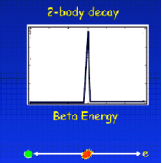
\includegraphics{decaimentobeta2corpos.png}
    \caption{Espectro de energia previsto pela teoria do Decaimento Beta.}
    \label{fig:my_label}
\end{figure}
Para encontrar o valor da energia máxima do elétron emitido pelo decaimento, a conservação de energia e do momento linear foi aplicada, encontrando a relação 

\begin{equation}
    E = ((m_A^2-m_B^2+m_e^2)/〖2m〗_A )c^2
\end{equation}
Onde a energia E é fixada.
Uma vez que as massas, mA, (massa do núcleo pai), mB (massa do núcleo filho) e me (massa do elétron), forem especificadas, esta energia seria exatamente o valor no pico do espectro esperado pela teoria do Decaimento Beta (fig. 1.1). No entanto, em 1914, J. Chadwick mediu experimentalmente o valor da energia do Decaimento Beta, seu resultado, figura 1,2, causou um enorme choque na comunidade científica
\begin{figure}
    \centering
    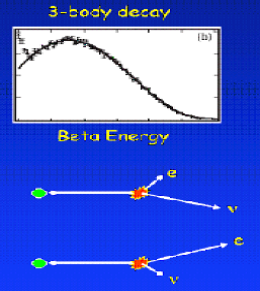
\includegraphics{verdadeirodecaimentobeta.png}
    \caption{Espectro de energia do Decaimento Beta medido experimentalmente.}
    \label{fig:my_label}
\end{figure}

O espectro encontrado por J. Chadwick, foi continuo sendo característico de um processo de três corpos. No entanto, para a teoria não existia um terceiro componente neste processo, inúmeros cientistas renomados chegaram a postular que a conservação da energia e momento linear não era válida para processos nucleares. Entretanto em 1930 Wolfgang Pauli postulou uma terceira partícula no processo5, trazendo assim uma nova luz sobre os resultados que Chadwick produziu. Esta nova partícula ficaria com a metade da energia do elétron, teria uma carga nula e mais tarde se mostrou que este novo corpo respeitaria a estatística de Fermi-Dirac, sendo assim, teria spin ½.Juntamente com o átomo filho (B) e o elétron, formariam um sistema de três corpos, o que seria um modelo aceitável para os resultados experimentais. Esta nova partícula foi denominada de neutrino (\nu).

\begin{figure}[!h]
\centering
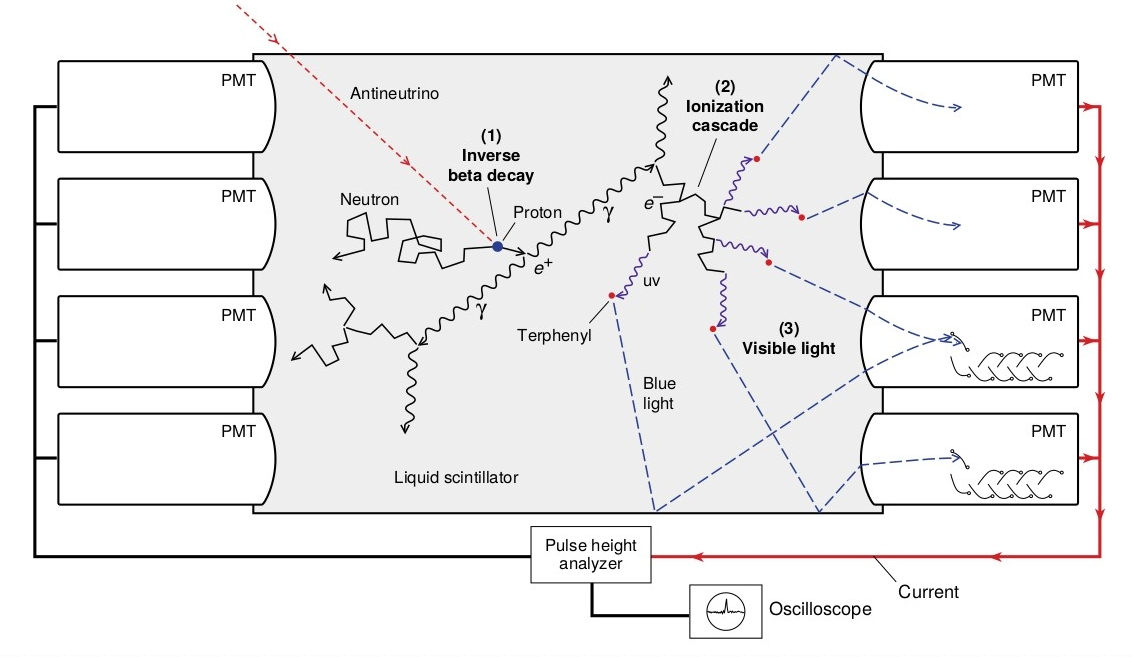
\includegraphics[scale=0.35]{sinal_antineutrino.jpg}
\caption{ A noite eh fria e cheia de terrores \cite{GRIFFITHS}. }
\label{fig:sinal_antineutrino}
\end{figure} 
\section{nome da seção}
\subsection{nome da subseção}
Texto.....